\clearpage
\section{MCU} \label{section:mcu}

This chapter describes the modules that execute on the MCU. The MCU is
responsible for supplying the FPGA core \todo{FPGA core name here} with audio
samples. It also has to receive the results coming from the FPGA core after the
audio processing has taken place. In order to provide the samples from input and
output, the MCU controls a variety of input/output peripherals.

The software responsible for this is implemented on a Giant Gecko ARM Cortex-M3
microcontroller, manufactured by Silicon Labs. This MCU is a complete miniature
computer on a single chip. Due to the energy saving features, along with a
generally low power consumption, of this MCU is a good fit with the overall goal
of this project, namely energy efficiency.


\subsection{Energy Efficient Software}

The software layer provides the most potential for energy savings, as the best
way to save power is to turn off the system completely. This descision is made
by the algorithm used. Still, a few techniques ensures that savings are posible even when the system 
is running. The most commonly know technique are {\bf interrupts}, in contrast to busy 
waiting. {\bf Sleep modes} are used for turning of parts of the system while still enabling 
some processing. {\bf DMA}, Direct Memory Access, enables movement of data while the
CPU is sleeping. 

The Giant Gecko provides 5 execution modes, where 4 modes are different levels of sleep. 
For this project sleep modes EM0, EM1 and EM3 was utilized.


\begin{description}
	\item[Energy Mode 0] - Run Mode \hfill \\
		Fully operational with all features available, used when handling interrupts and while reading from SDCard.
	\item[Energy Mode 1] - Sleep Mode \hfill \\
		CPU turned off, used when the system is performing filtering, required by EBI.
	\item[Energy Mode 3] - Stop Mode \hfill \\
		Deepest sleep mode without reset required, used when Bitless is idle.
\end{description}
Refere to the user manual for addition information \ref{}.


% !TEX root = ../../../report.tex

\subsection{Software Architecture}

All the software used in the project is based on the CMSIS \cite{cmsisapi} code
base from ARM. The Giant Gecko MCU is supplied with a peripheral API, called
emlib \cite{emlibapi} which builds upon CMSIS and can be used to initialize and
control all attached peripherals. The project code and programming model is
based on the structure in emlib, see Figure \ref{fig:software-stack}.

\begin{figure}[H]
    \centering
    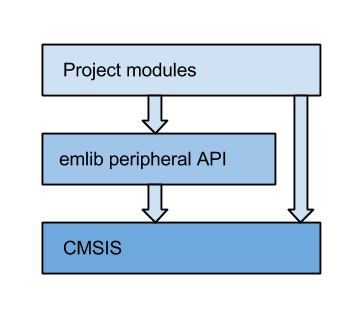
\includegraphics[height=150px]{figures/sw/software-stack.png}
    \caption{The software stack used on the microcontroller}
    \label{fig:software-stack}
\end{figure}


The application code is structured into directories representing each of the
modules, or peripherals, which have custom software written for it. Each module
contains three directories, \textit{inc}, \textit{src} and \textit{demo}.
These directories contains header files, source files, and different demos and
test programs for the modules. Each module is typically implemented as a
combination of a driver and a controller, for the peripheral it is designed for.

The custom library for Bitless includes code for setting up and controlling
all the peripherals described in the following sections.

% application
% emlib
% cmsis
%!TEX root = ../../../report.tex

\subsection{Dataflow}
When designing an energy efficient system, dataflow is of great importance. The
software on the MCU has been designed to minimize the number of data-stores and
-movements. When possible, DMA is utilized to move the data while running the
MCU in a low power mode. The dataflow consist of four phases, as shown in figure
\ref{sw_transfer_phases}.

In phase 1 the MCU acquires input samples from an input device. These samples
are then transferred to the FPGA in phase 2. When the FPGA is finished
processing the samples, they are transferred back to the MCU in phase 3. In the
last phase, the MCU sends the filtered samples to an output device. All these
phases are executed concurrently to ensure a constant flow of samples.

\begin{figure}[H]
	\centerline{
	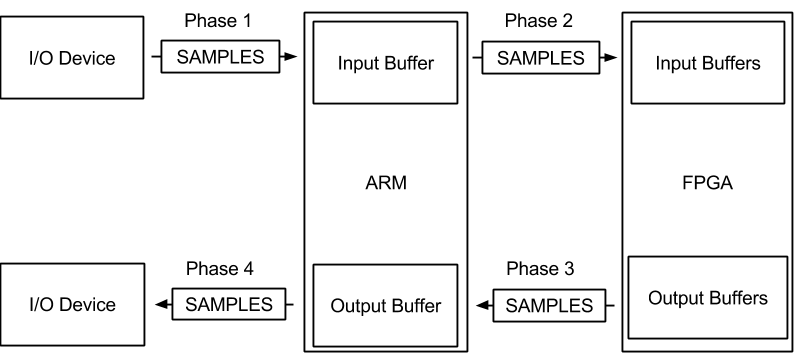
\includegraphics[width=400px]{figures/sw/transfer-phases.png}}
	\caption{Transfer Phases}
	\label{fig:sw_transfer_phases}
\end{figure}
\FloatBarrier


\subsubsection{Direct Memory Access}
Drect Memory Access (DMA) provides the ability to move data
without the intervention of the CPU. This is used extensively to implement the
dataflow when the MCU is running in a low energy mode. The CPU is only used to configure
and refresh the DMA channels in between transfers. The MCU provides 12
independent DMA channels which can move data between peripherals, Internal RAM, and
devices connected to EBI, like the FPGA.

The main flow of data goes from Internal RAM in the MCU to the buffers on
the FPGA, and back to Internal RAM in the MCU. This dataflow path is illustrated in \todo{which figure??}figure.

% \input{figures/sw/ram-fpga-ram}

\paragraph{Deinterleaving of Samples}
When reading from both a WAV file or the ADC, samples from the stereo channels
are interleaved. The FPGA handles each channel in a separate pipeline as shown
in figure \ref{fig_sw_main_dataflow}.
When reading the samples they have to be deinterleaved. Deinterleaving is the
process of splitting the samples for each channel into separate streams.
The complementary operation of interleaving the samples is performed before the samples
are moved to the output peripherals.
\missingfigure{Figure showing deinterleaving and interleaving}

The interleaving and deinterleaving operations are either done by the DMA for
energy efficiency purposes, or the CPU on the MCU. If the operation is performed
by the CPU, the gains of speed and data-transfer analysis can be tested. Depending
on the different types of input sources, the CPU is needed on some occasion, while
on others a more energy efficient implementation through the use of DMA may be used.
Comparions of the two implementations are included in the results section.

The samples are deinterleaved in the DMA implementation by letting two DMA channels read from the
same source and write the correct channel into the the correct pipeline for the correct channel.
The first DMA copies the samples for the left stereo channel, and starts without a offset. The
second DMA copies the samples for the right stereo channel and starts with an
offset of one sample. Both DMAs read every other sample and writes them
continuously to the FPGA input buffers.

In code this is setup with the DMA interface in {\bf emlib}.

\begin{lstlisting}
  DMA_CfgDescr_TypeDef descrCfg = {
    .dstInc  = dmaDataInc2,
    .srcInc  = dmaDataInc4,
    .size    = dmaDataSize2
  };
  DMA_CfgDescr( DMA_FPGA_IN_LEFT,  true,  &descrCfg );
  DMA_CfgDescr( DMA_FPGA_IN_RIGHT, true,  &descrCfg );
\end{lstlisting}
To understand what this will result in, imagine two pointers, {\bf dst} and {\bf src}.
At each iteration {\bf size} bytes are copied from {\bf src} to {\bf dst}. After each
iterations the {\bf src} pointer is incremented by {\bf srcInc} bytes and the {\bf dst}
pointer is incremented by {\bf dstInc}.

After the DMA channel is configured with a descriptor, it can be started with a
a source pointer, destination pointer, and the number of transfers to be executed.
When the transfer has finished the CPU is interrupted and can start the next transfer.

The interleaving process on the output side of the FPGA works in the same way. The DMA reading
the audio pipeline containing the left stereo channel, writes the samples to even numbered
addresses in the memory, while the DMA reading the right audio pipeline channel writes
to odd numbered addresses.

\paragraph*{}
In addition, a DMA is assigned for each ADC and DAC whenever they are used as
input and output. When a SDCard is used, the contents of the files are read and
written directly to and from RAM by the CPU.

\subsubsection{Peripherals}

\begin{figure}[h]
	\centering
	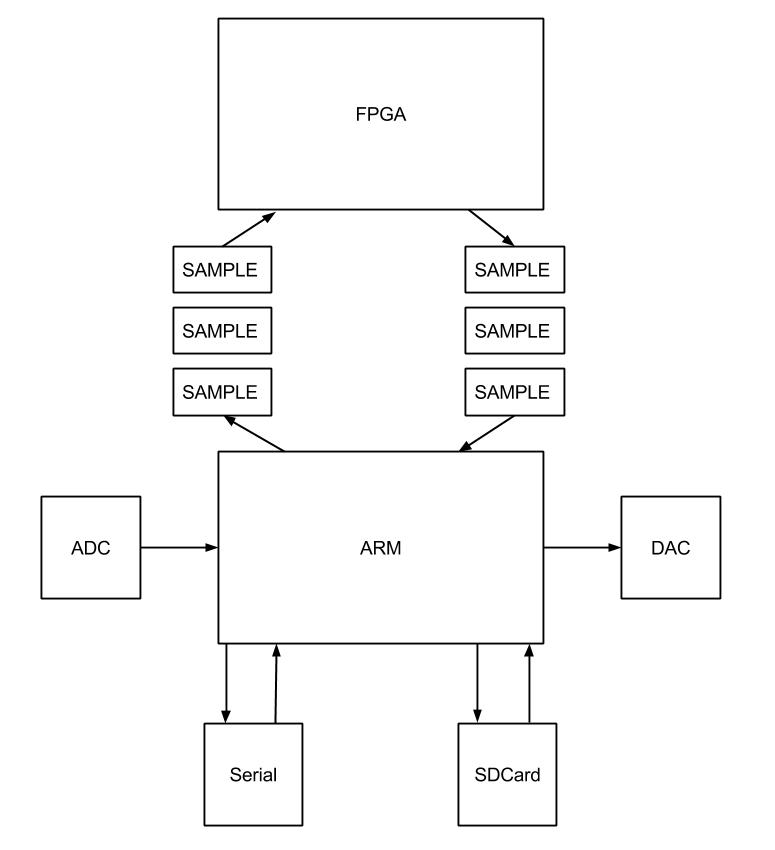
\includegraphics[height=150px]{figures/sw/sample-flow.png}
	%\begin{tikzpicture}[shorten >= 1pt, node distance=3cm, on grid, auto]
	%	\node[draw,rectangle,minimum size=2cm] (fpga) {FPGA};
	%	\node[draw,rectangle,below of=fpga,minimum size=2cm] (arm) {ARM};
	%\end{tikzpicture}
	\caption{Flow of samples}
	\label{fig:sw_sample_flow}
\end{figure}
\todo{Tikzify}


Figure \ref{fig:sw_sample_flow} shows all the peripherals included in the flow of samples.
The ADC and DAC are connected to the minijack audio ports on the circuit board and directly
linked to GPIO ports on the MCU. The SDCard
is mounted on the PCB and connected to the MCU through the Serial Peripheral Interface (SPI)
bus. Lastly the FPGA is connected to the MCU on the EBI.

\subsubsection{External Bus Interface}
The MCU is connected to the FPGA and External SRAM through the EBI. The EBI bus
is initialized by the {\it emlib} software library. Utilizing
the EBI leads to a simple interface with these units since the bus is memory
mapped on the MCU. Communicating with the FPGA is done by reading and writing to memory.

\subsubsection{Serial Peripheral Interface}
The SPI bus is a general bus interface used in many embedded applications. It is used
for communication between the MCU and a MicroSD memory card connected to the slot
on the PCB \ref{} \todo{Har vi bilde av bitless?}.

\subsubsection{General Purpose Input/Output}
To capture an audio stream from the input minijack, one GPIO pin is connected to an
ADC on the MCU. The ADC measures the the

\todo{more about how the bus is implemented on the MCU}

\paragraph{Triggering Transfers}

All the DMA transfers are triggered by the use of one clock, the sample clock.
This clock is run at the sample speed 11 kilohertz when using the DAC or ADC. Or
an arbitrary frequency when sampling from SDCard to SDCard. The clock signal is fed into
the Peripheral Reflex System \todo{Refere to manual} (PRS) of the MCU and propagates
through the system using the following scheme.

%\newpage %re-insert if figure breaks across pages
\begin{verbatim}
                        | Audio in
                        V
+------+  +-----+    +------+   +-----+     +--------+
|TIMER0|->| PRS |-+->| ADC0 |-->| DMA |---->| Buffer |
+------+  +-----+ |  +------+   +-----+     +--------+
                  |     .                      / \
                  |     .                     /   \
                  |     .                    V     V
                  |     .              +-----+     +-----+
                  |     +....irq......>| DMA |....>| DMA |
                  |                    +-----+     +-----+
                  |                       |           |
                  |                       V           V
                  |                   +------+    +-------+
                  |                   | FPGA |    | FPGA  |
                  |                   | Left |    | Right |
                  |                   +------+    +-------+
                  |                       |           |
                  |                       V           V
                  |                    +-----+     +-----+
                  |     +....irq......>| DMA |....>| DMA |
                  |     .              +-----+     +-----+
                  |     .                    \     /
                  |     .                     \   /
                  |     .                       V
                  |  +------+   +-----+     +--------+
                  +->| DAC0 |<--| DMA |<----| Buffer |
                     +------+   +-----+     +--------+
                        |
                        V Audio out
\end{verbatim}

Here, both the DAC and ADC consumes the PRS signal originated from TIMER0. The
DMA copying from the ADC to the RAM buffer, as well as the two DMAs performing the
deinterleaving of the input samples, both receive a pulse each time the ADC has
buffered $N$ samples. They then perform a sequence of copy actions on the input
samples so that these end up inside the pipeline bufferrs of the FPGA. On the
other side, the DAC sends a pulse to the DMA that feeds it samples in conjunction
with the two DMAs performing the interleaving of the samples returned from the
FPGA pipelines.

% peripherals+modes (sdcard, dac, adc, serial?)
% ebi (FPGA + SRAM)
% dma
\input{chapters/implementation/mcu/userio}
% serial
% button and leds
